\chapter{Transactions}

The Storage Engine offers features aimed at solving recovery and concurrency problems, guaranteeing that each operation performed by the user is executed such that the user does not notice any underlying failure, and that there are no interferences with other operations running concurrently. The solutions to these problems are based on a mechanism called \textbf{transaction}.
\BoxDef{Transaction}{
    A transaction is a sequence of operations on the database and on temporary data, with the following properties:
    \begin{itemize}
        \item Atomicity: only successful transactions change the state of the database; if a transaction is interrupted the database must remain unchanged as if the transaction was never started;

        \item Isolation: when a transaction is executed concurrently with others, the final effect must be the same as if it was executed alone;

        \item Durability: the effects of committed transactions must survive system and media failures.
    \end{itemize}
}
Often, the acronym \textbf{ACID} (\textbf{Atomicity}, \textbf{Consistency}, \textbf{Isolation}, and \textbf{Durability}) is used to refer to the properties of transactions. The Recovery Manager ensures Atomicity and Durability, while the Concurrency Control Manager ensures Isolation. Consistency is guaranteed by the implementation of integrity constraints and code correctness.

For the DBMS, a transaction $T$ requires a number of read/write operations on the database. Each transaction starts and ends with the following transaction operations:
\begin{itemize}
    \item \textit{beginTransaction}, signaling the start of the transaction;
    \item \textit{commit}, signaling the successful termination of the transaction, and requiring the system to make its updates durable;
    \item \textit{abort}, signaling the abnormal termination of the transaction, requiring the system to undo its updates.
\end{itemize}
While a \textit{commit} is only used as a command in the code, \textbf{abort} can be either specified in the code or it can be used by the system. The execution of a \textbf{commit} does not automatically mean that the transaction will successfully terminate, because its updates may not be written on permanent memory. Figure \ref{fig:transaction-states} shows the state transition diagram for transaction execution.
\begin{figure}[h]
    \centering
    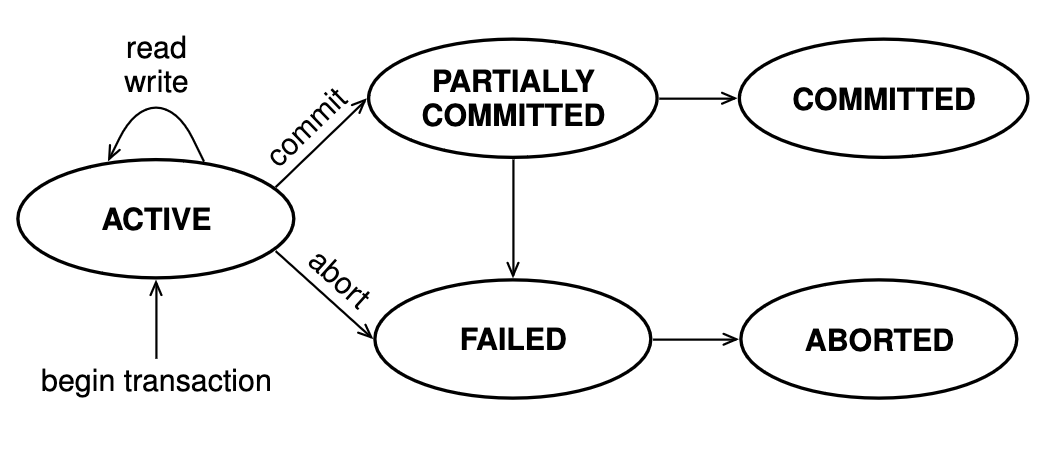
\includegraphics[width=0.5\linewidth]{img/transaction_states.png}
    \caption{State transition diagram for transaction execution.}
    \label{fig:transaction-states}
\end{figure}
To read a page ($r_i[x]$), it is brought into the buffer from the disk (if it's not already in the buffer), and then read. To write a page ($w_i[x]$), an in-memory copy is modified, which will later be written to disk when the Buffer Manager find it appropriate to do so. This delayed writing has to be compatible with Atomicity and Durability, since multiple transactions may want to write to the same page.

\section{Failures}

A database can become inconsistent because of three types of failures:
\begin{itemize}
    \item \textbf{Transaction failure}, an interruption of a transaction which does not damage the content of either the main memory or the permanent memory. A transaction can be interrupted because either it meets certain conditions, it violates integrity constraints, or the concurrency manager chooses to abort it because it is involved in a deadlock;
    
    \item \textbf{System failure}, an interruption (crash) of the system (DBMS or OS) in which the content of the main memory is lost, but the content of the content of the permanent memory remains intact. After crashes occur, the system is restarted, automatically or by an operator;
    
    \item \textbf{Media failure} (also called \textbf{disaster}), an interruption of the system in which content of the permanent memory is lost or damaged. When a media failure happens, the Recovery Manager uses a backup to restore the database.
\end{itemize}
Other than database backups, another protection from failures is represented by \textbf{log files}: these files contain lines recording each transaction operation executed in the system, including aborted transactions. For each transaction, the information written is when it starts, when it commits, when it aborts, and when it modifies a records, specifying the page the record is in, and the old and new values (called \textbf{before image} and \textbf{after image}). Each record is uniquely identified by a LSN (Log Sequence Number), assigned in a strictly increasing order.

A recovery algorithm requires an \textbf{undo} if an update of some committed transaction is stored in the database. An \textit{undo} is needed when a transaction or system failure occurs, copying the before image of the page from the log to the database. A recovery algorithm requires a \textbf{redo} is a transaction is committed before all of its updates are stored in the database (after a system failure), copying the after image in the log to the database.

The downtime of the system is given by the product between the failure rate and the recovery rate. The failure rate cannot be reduced, as we cannot know in advance if a transaction contains an error, or a system/media failure happens. The way to reduce downtime is to reduce recovery time. In practice, this is done via \textbf{checkpoints}. There's different types of checkpoints:
\begin{itemize}
    \item \textbf{Commit-consistent checkpoint}: when a checkpoint starts, the activation of new transactions is suspended, and the system waits the termination of active transactions; all ``dirty'' pages in the buffer are written to permanent memory; the checkpoint is written to the log file, and a pointer to the corresponding record is stored in a special file called \textbf{restart file}. The system then resumes normal activity. This strategy is simple but inefficient, since the system has to regularly stop.

    \item \textbf{Buffer-consistent checkpoint - Version 1}: similar to the previous type, but once the checkpoint starts, it also suspends the execution of currently active transactions. This strategy is more efficient than the previous, but it is still slow because of the buffer flushing operations.

    \item \textbf{No stop checkpoint}: once the checkpoint starts, the checkpoint is written to the log file, along with the ids of currently active transactions; a new thread is started, which scans the buffer and flushes the dirty pages it finds in parallel with the standard transactions, guaranteeing that all pages that were dirty at the beginning of the checkpoint are flushed before its end.
\end{itemize}

\subsection{Recovery from System and Media Failures}

In order to recover the database, the \textit{restart} operator is invoked, bringing the database in its committed state with respects to the execution up to the system failure, and restarting the normal system operations. The first task is done using a recovery algorithm of which a simple version will be described. This algorithm has two phases, \textbf{rollback} and \textbf{rollforward}. In the rollback phase the log is read backwards, to undo updates of transactions that were not terminated before the crash, and to find the identifiers of the transactions which terminated successfully. In particular, two sets are constructed: the \textbf{redo-list} and the \textbf{undo-list}. Until the first checkpoint record is found, these operations are done:
\begin{enumerate}
    \item If a record is (\textit{commit}, $T_i$), $T_i$ is added to the redo-list.
    
    \item If a record is an update of a transaction $T_i$ not in the redo-list, it is added to the undo-list.

    \item If a record is (\textit{begin}, $T_i$), $T_i$ is removed from the undo-list.

    \item If a record is a checkpoint (\textit{CKP}, $L$), for each $T_i \in L$ if $T_i$ is not in the redo-list it is added to the undo-list. If the undo-list in not empty, the rollback phase continues until it is completely emptied.
\end{enumerate}
In the rollforward phase, the log is read onward from the first record after the checkpoint, redoing all operations of the transactions in the redo-list.

The restart is executed at the buffer level, not on the persistent store: undos and redos are done by first loading the data in the buffer, and then pages are eventually flushed in a second time.

The algorithm described above is the standard Undo-Redo algorithm, but there exist variants:
\begin{itemize}
    \item \textbf{NoUndo-Redo}: requires that all the updates of a transaction must be in the database after the transaction has committed. It uses a \textbf{NoSteal (Pin) Policy}, where all the buffers used by transactions are pinned, and those pages will not be flushed to disk until the transaction commit. This way, no operation ever needs to be undone. It is dangerous because it pins all those pages used by the active transactions, limiting the freedom of the buffer manager.

    \item \textbf{Undo-NoRedo}: requires that all the updates of a transaction must be in the database before the transaction has committed. It uses a \textbf{Force} policy, where buffer pages used by transactions are forcibly flushed before committing. This approach has two problems: it does not work for media failures, and it is costly since it requires a lot of writes to disk.

    \item \textbf{NoUndo-NoRedo}: requires that all the updates of a transaction must be in the database neither before nor after the transaction has committed. It uses NoSteal and Force policies.
\end{itemize}
Undo-Redo uses Steal and NoForce policies.

NoUndo-NoRedo requires a way to write many pages atomically. This is done using \textbf{shadow pages}. When a transaction updates a page for the first time, a new database page is created, called \textbf{current page}, with a certain address $p$. The old page in the database is unchanged, and becomes a shadow page. The \textbf{New Page Table} (a copy of the Page Table containing all physical addresses of pages) is updated so that the first element contains the physical address $p$ of the current page. All subsequent write and read operations on that page will operate on the current page.

Once the transaction reaches the commit point, the system substitutes all shadow pages with an atomic actions: first, all the pages updated in the buffer are written to the permanent memory, while the Page Table is left unchanged; then, the descriptor of the database is updated with an atomic operation, replacing the pointer to the Page Table with that to the New Page Table, which becomes the Page Table.

There are some optimizations of the algorithm:
\begin{itemize}
    \item Setting the log granularity at a record level instead of page level;

    \item Buffering the log;

    \item Writing in pages the LSN of the last operation executed;

    \item Logging undo actions;

    \item Adding to each log entry the LSN of the previous entry for the same transaction.
\end{itemize}